\chapter{Atividades Realizadas}

\section{Protótipo das implementações do método}
A implementação do método foi toda feita utilizando orientação a objetos em C++, com excessão das funções específicas ao cálculo que possuem implementações, em CUDA, OpenCL e C++. Estas funções específicas ao cálculo consistem de operações básicas com vetores, aproximações para o campo vetorial e o método de Runge-Kutta em si. O código compartilhado entre as demais implementações vai desde as estruturas de dados até representações dos resultados em OpenGL.

O código pode ser encontrado em seu repositório Git \newline(em \href{https://github.com/rafamanzo/runge-kutta}{https://github.com/rafamanzo/runge-kutta}) é organizado basicamente em quatro pastas:
\begin{itemize}
  \item \textbf{core} contém as três implementações do método nas pastas \textit{c}, \textit{cuda} e \textit{opencl}; além das estruturas de dados que repensentam a entrada (\textit{dataset.cpp}) e a saída do método (\textit{fiber.cpp}).
  \item \textbf{example-factories} contém os scripts que geram arquivos de entrada para o protótipo de campos vetoriais sintéticos como exemplos;
  \item \textbf{includes} contém todos os cabeçalhos necessários, facilitando sua inclusão;
  \item \textbf{io} contém as classes que cuidam da entrada e saída do protótipo. A pasta \textit{gui} contém as abstrações utilizadas para a criação de uma interface gráfica com Glut e OpenGL.
\end{itemize}

\newpage
As interações entre todas as classes que compõe o protótipo podem ser vistas através do seguinte diagrama de classes:
\begin{figure}[!h]
  \begin{center}
    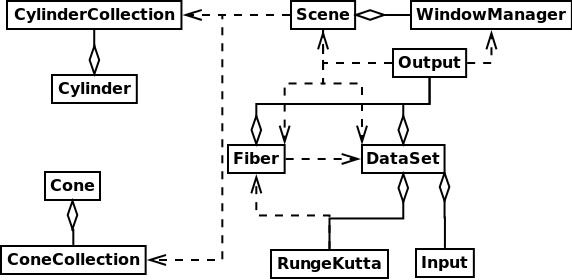
\includegraphics[width=120mm, height=60mm]{images/diagramadeclasse.png}
    \label{fig:}
    \caption{Diagrama de classes simplificado para o protótipo}
  \end{center}
\end{figure}

  \subsection{Estruturas compartilhadas em C++}
  A estrutura mais básica é a \textit{vector} contida em \textit{include/dataset.h}, consistindo de três \textit{doubles}. Sua responsabilidade é representar tanto vetores quanto pontos no $\Re ^{3}$. Neste mesmo arquivo também está a representação da classe \textit{DataSet}, cujo uso é representar as informações de entrada referentes ao campo vetorial e encapsular seu acesso. Analogamente, a classe \textit{Fiber} é responsável por representar os resultados da aplicação do algoritmo.
  
  Além destas abstrações de entrada e saída, existem classes que de fato são responsáveis pela entrada e saída do protótipo. A mais simples é a classe que cuida da entrada, \textit{Input}, que possui os métodos para ler um arquivo de texto que contenha as informações sobre o campo vetorial, pontos iniciais e tamanho de passo (conforme descrito no arquivo \textit{README} que acompanha o protótipo). Outra opção de entrada é o formato Analyze que é suportado pelo biblioteca $\textit{CImg}_{\ref{CImg}}$ e portanto o método da classe \textit{Input} que processa este tipo de entrada apenas faz uma chamada a esta biblioteca.
  
  Por fim, a última estrutura compartilhada entre as três implementações é a saída. A forma mais simples de visualizar os resultados é através do $\textit{gnuplot}_{\ref{gnuplot}}$ passando para este o arquivo \textit{rk2-vs-rk4} que é criado ao fim da execução do algoritmo. Por outro lado, a saída pode ser bastante mais complexa que apenas uma classe, como é a entrada, devido à visualização com \textit{Glut} e \textit{OpenGL}.
  
  Esta visualização é composta das classes, aqui denomidas como primitivas, contém representações de cilindros e cones (classes \textit{Cylinder} e \textit{Cone}) e as responsáveis por representar coleções destas classes (\textit{CyllinderCollection} e \textit{ConeCollection}). Estas classes primitivas contém principalmente informações sobre como renderizar estes objetos.
  
  Por fim, ainda na interface gráfica, existe a classe \textit{Scene} que é responsável por fornecer métodos que utilizam as primitivas para evitar que a classe \textit{WindowManager} use diretamente as primitivas e tenha que conhecer suas especificidades. Ou seja, ela é como uma camada de abstração para a \textit{WindowManager}, permitindo que esta seja responsável apenas pela interação com a \textit{Glut}. 
  
  \subsection{Implementação do método}
  A implementação em cada linguagem pode ser encontrada nas subpastas de \textit{core} (\textit{c}, \textit{cuda} e \textit{opencl}), nos arquivos \textit{rk\_kernel.*} aos quais iremos nos referir apenas como \textit{kernel}. Também cada uma destas pastas contém um arquivo \textit{rk.cpp} reponsável por fornecerer uma interface para seu respectivo \textit{kernel}.
  
  Estas interfaces são utilizadas pois a implementação, por limitação do \textit{CUDA} e do \textit{OpenCL}, não pode ser feita utilizando orientação a objetos. Então a classe (\textit{RungeKutta}) implementada no arquivo \textit{rk.cpp} é a responsável por encapsular o conjunto de funções definidas em seu respectivo \textit{kernel}.

  Cada arquivo de \textit{kernel}, além de conter a implementação do método, possui funções auxiliares para se trabalhar com elementos do $\Re ^{3}$ (soma, subtração, módulo, distância e produto por um escalar) e as funções de aproximação necessárias (\ref{aproximacao}).
  
  Com todo esta estrutura descrita, o método em si é a simples implementação do que é descrito para as ordens 2 e 4 na seção \ref{rungekutta} com especificidades para as diferentes linguagens utilizadas descritas a seguir.
  
  Antes é preciso destacar que todas as implementações de diferentes ordens são funções independentes umas das outras e que, para evitar que falte memória, os resultados foram limitados a 10000 pontos que podem ser gerados a partir de cada ponto inicial.
  
    \subsubsection{Observações sobre o método em C++}
    Esta implementação, ao contrário das demais, foi feita sequencial e apenas não foi feita orientada a objetos para seguir a arquitetura necessária para as outras duas implementações.
    
    \subsubsection{Observações sobre o método em CUDA}
    Nesta implementação para \textit{GPU}, além do limite de 10000 pontos que podem ser gerados por cada ponto, é feita uma rechecagem após alocar toda a memória necessária para o \textit{DataSet} calculando novamente a quantidade máxima de pontos que podem ser gerados a partir de cada ponto inicial baseado na memória dedicada que restou. Então, o limite é o mínimo entre 10000 e este valor calculado.
    Outro ponto importante de destacar é que a chamada é feita com apenas um bloco contendo uma \textit{thread} para cada ponto inicial sobre o qual o algoritmo deverá ser aplicado.
    
    \subsubsection{Observações sobre o método em OpenCL}
    
  \subsection{Geração de campos vetoriais sintéticos}

\section{Protótipo das implementações utilizando a biblioteca VTK}
\section{Abstrações da VTK para uso de CUDA e OpenCL}
\section{Integração com o MedSquare através do VTK}
